\documentclass[11pt]{article}
\usepackage[utf8]{inputenc}
\usepackage{graphicx}
\graphicspath{ {./images/} }
\usepackage[
backend=biber,
style=numeric-comp,
sorting=ynt
]{biblatex}

\addbibresource{sources.bib}

\title{Twofish Cipher}
\author{Jorge Contreras}
\date{May 2022}


\begin{document}
\maketitle


\begin{abstract}
Twofish was one of the AES competition's finalists. Although it was not picked as the winner, it is fascinating to investigate and comprehend how any of these ciphers operate. This paper will explore and focus on Twofish; however, the other finalists, Rijndael, Serpent, RC6, and MARS will be often mentioned as they are also part of the historical background of Twofish. The goal is to understand the basic engineering behind Twofish, the process of encryption, and then compare its performance, pros and cons, against the other finalists to get a better understanding in why NIST ultimately chose Rijndael as the AES.
\end{abstract}



\section{Introduction}
Twofish is a symmetric-key block cipher that uses a block size of 128 string of bits, and takes keys of up to 256 bits in length. It was a finalist in the Advanced Encryption Standard competition during the late 90s, however the National Institute of Standards and Technology (NIST) chose Rijndael, which is also a block cipher, for standardization. Twofish was designed by the cryptographers Bruce Schneier (who also designed Blowfish, an early  symmetric-key block cipher), John Kelsey, Doug Whiting, David Wagner, Chris Hall, and Niels Ferguson.

Twofish accepts key lengths of 128 bits, 192 bits, and 256 bits and has asimple design, both to facilitate ease of analysis and ease of implementation \cite{schneier1999twofish}. It was able to encrypt data in less than 500 clock cycles per block on an Intel Pentium, Pentium Pro, and Pentium II, for a fully optimized version of the algorithm \cite{schneier1999twofish}.

\section{Design}

\subsection{Block Cipher}
Twofish is a symmetric-key block cipher which means that the data is both encrypted and decrypted using only one secret key. This key must be exchanged between the parties communicating so that it may be utilized in the decryption process. Stream ciphers encrypt data one bit or byte at a time, in contrast, Twofish processes fixed-size blocks at the same time.

\subsection{Feistel Network}
In addition, Twofish uses a specific type of block cipher construction known as Feistel cipher or Feistel network. A Feistel network is a general method of transforming any function (usually called the F function) into permutation \cite{schneier1999twofish}. 

The F function is the most basic component of a Feistel network. This is a key-dependent mapping of an input string to an output string. This can be visualized by the formula:
\begin{equation}
F : \{0, 1\}^{n/2} \times \{0, 1\}^N \to \{0, 1\}^{n/2}
\end{equation}
where n is the Feistel network's block size, and F is a function that takes \(n/2\) bits of the block and N bits of a key as input and produces an output of length \(n/2\) bits \cite{schneier1999twofish}. The "source block" is the input to F in each round, and the "target block" is \(XOR\)ed with F's output, then after these two blocks switch places for the following round. 

In a Feistel network, two rounds are one cycle and in each cycle every bit of the text block has been modified once. Twofish uses this mechanism as it is a 16-round Feistel network.

\subsection{S-boxes}

In most block ciphers, an S-box is a table-driven non-linear substitution process. It performs replacement and is a fundamental component of symmetric key algorithms. They are commonly employed in block ciphers to obscure the relationship between the key and the ciphertext. S-boxes have variable input and output sizes and can be generated either randomly or algorithmically. 

Twofish employs four key-dependent 8-by-8-bit S-boxes. These S-boxes are constructed with two fixed 8-by-8-bit permutations and key material.

\subsection{Others tools}

Twofish additionally uses MDS matrices for diffusion, Pseudo-Hadamard Transforms (PHT), Whitening, and Key Schedule. A Pseudo-Hadamard transform is a simple mixing operation that can be performed in software quickly. Given two inputs, a and b, the 32-bit PHT is defined as:
\begin{equation}
a' = a + b\ mod\ 2^{32}
\end{equation}
\begin{equation}
b' = a + 2b\ mod\ 2^{32}
\end{equation}
Twofish uses a 32-bit PHT to mix the outputs from its two parallel 32-bit g functions \cite{schneier1999twofish}.

Whitening is the technique of \(XOR\)ing key material before the first round and after the last round. This increases the
difficulty of keysearch attacks against the cipher. The key schedule is the process of converting key bits into round keys that the cipher can use. The round function and the key schedule both use the same primitives.

\section{The Twofish Cipher}
In figure 1 it can be seen how the Twofish cipher works. Twofish employs a Feistel-like 16-round structure and uses whitening of the input and output. The plaintext is broken down into four 32-bit words. These are \(XOR\)ed with four key words during the input whitening step. This is then followed by sixteen rounds. The plaintext is broken down into four 32-bit words. These are \(XOR\)ed with four key words during the input whitening step. One of them is first rotated by 8 bits. The g function is made up of four byte-wide key-dependent S-boxes, which are followed by a linear mixing step based on an MDS matrix.

\begin{figure}[t]
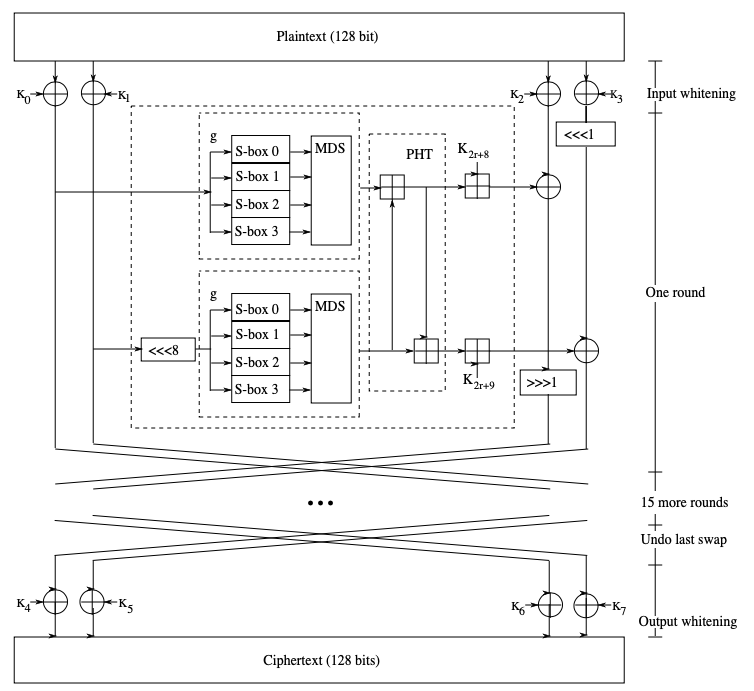
\includegraphics[width=\textwidth]{images/twofish}
\caption{Visual representation of the Twofish cipher \cite{schneier1999twofish}}
\end{figure}

A Pseudo Hadamard Transform is used to combine the results of the two g functions and two keywords are added. These two outcomes are then \(XOR\)ed into the words on the right. One is rotated left by one bit first, and the other one follows with a right rotation. For the next round, the left and right halves are switched. After all rounds, the last round's swap is reversed, and the four words are \(XOR\)ed with four additional key words to generate the ciphertext.

To summarize, the 16 bytes of plaintext are first divided into three 32-bit words. These words are then \(XOR\)ed with four words from the enlarged key during the input whitening stage. The first two words are used as input to the function F in each of the 16 rounds, which also uses the round number as input. The third word is \(XOR\)ed with the first F output before being rotated right by one bit. The fourth word is \(XOR\)ed with the second output word of F after being rotated left by one bit. Finally, the halves are swapped. The output whitening step reverses the previous round's swap and \(XOR\)s the data words with the expanded key's four words and the four ciphertext words are then encoded as 16 bytes.

\section{Performance}
In order to measure the performance of Twofish, other ciphers need to be mentioned. Twofish was one of the five finalists of the Advanced Encryption Standard contest, but it was not selected for standardization.

According to the Twofish designers ``It is easy to design a secure algorithm by ignoring performance. It is also easy to make an algorithm faster by reducing its security" \cite{schneier2000twofish}. Many believe that Twofish should have been the winner of the AES competition as this cipher has been claimed to be more secure than Rijndael but not faster. In fact the the designers wrote a final paper after examining their competitors and they claim that Twofish offers the best security/performance tradeoff of all the AES finalists, and urge NIST to choose Twofish as the single AES standard \cite{schneier2000twofish}.

In 2001 Dr. Stefan Lucks claimed to have developed the best known attack on Twofish by using a saturation attack and ``break up to 8 rounds of Twofish with one-sided whitening faster than exhaustively searching the key would require" \cite{lucks2001saturation}. Nonetheless, this attack would be able to penetrate one half of Twofish leaving it with still a decent security margin.

In addition, Bruce Schneier and Doug Whiting mention on their ``A Performance Comparison of the Five AES Finalists" paper that more interesting than individual performance measures is the ratio of safety factor to performance of the AES finalists. When ``looking at the five algorithms in this manner—normalizing to the largest number of rounds cryptanalyzed is a reasonable metric, Twofish far surpasses the other four finalists" \cite{schneier2000performance}.

According to NIST, Rijndael and Serpent are the fastest in hardware encryption, Twofish is sufficient, while RC6 and MARS are both slower and expensive. On the other hand, Rijndael and Twofish are the quickest in software encryption, MARS and RC6 are decent, while Serpent is quite slow \cite{schneier2000twofish}. 

Furthermore, Twofish was designed to function well across a wide range of hardware and software systems, rather than being tailored for a single platform and executes at the same speed for encryption and decryption. Not to mention that optimization ``tricks" can be used to improve the performance of Twofish. For instance, the process would speed up if the round keys are compiled into the code. Despite Twofish being more secure than Rijndael, NIST ultimately chose Rijndael for standardization as it is both faster and simpler than Twofish.

\section{Conclusion}

NIST had strict criteria for choosing the AES. The requirements included the ciphers to be strong block ciphers, have a variable key size so that security could be increased when needed, be at least as secure as Triple DES, and be significantly more efficient than Triple DES. In addition, key sizes of 128 and 256 bits were mandatory, and key setup time would be important when considering the efficiency and the agility of the algorithm. 

Twofish is an interesting, complex cipher that could have been the winner of the AES contest. When studying modern ciphers and cryptography it is important to understand why Rijndael was chosen over the finalists and how do these ciphers work. There is not straightforward reason to answer why Twofish was not chosen as the finalist but after reviewing the cipher it can be concluded that due to the lack of power of machines and processors it seemed more efficient to choose a simpler cipher like Rijndael. It also should not be forgotten that Rijndael was tweaked and simplified before actually becoming the AES.

Twofish is still a strong cipher today. Since it uses a 128-bit key, a brute-force attack could still take decades to decrypt. Nonetheless, since Twofish encryption method employs pre-computed replacement this could make it vulnerable to side channel attacks. However, Bruce Schneier affirms that there are still not any true cryptanalysis attacks against Twofish.


\printbibliography


\end{document}
